%\section{Differentiability and Continuity}
\vspace{-0.25 in}
\begin{framed}
\subsection*{Objectives}
\begin{itemize}
    \item Be able to recognize when a function is not differentiable at a point.
    \item Be able to determine when a function is continuous at a point and/or over a specified interval.
    \item Be able to determine if a function has any points of discontinuity.
\end{itemize}

%%%Reading Assignment%%%
\subsection*{Suggested Reading:}
\begin{itemize}
\item \cite{Calaway}\footnotemark[1]
   \begin{itemize}
        \item \emph{Section 2.1 Limit and Continuity}
        \begin{itemize}
            \item Continuity 
        \end{itemize}
    \end{itemize}

\item \cite{openstax}\footnotemark[2]\textsuperscript{,}\footnotemark[3]
    \begin{itemize}
        \item \emph{Section 2.4 Continuity}
        \begin{itemize}
            \item Continuity at a Point
            \item Types of Discontinuities
            \item Continuity over an Interval
        \end{itemize}
    \end{itemize}
\item \cite{Hoffman}\footnotemark[3]\textsuperscript{,}\footnotemark[4]
    \begin{itemize}
        \item \emph{Section 1.3: Continuous Functions})
        \begin{itemize}
            \item Definition and Meaning of Continuous.
           \item Graphic Meaning of Continuity
            \item Why do we care whether a function is continuous?
            \item Which Functions Are Continuous?
        \end{itemize}
        
    \end{itemize}
\end{itemize}
%\subsection*{Supplemental Materials:}
%%%Key Terms%%%
\subsection*{Key Terms:} 

\begin{multicols}{2}
\begin{itemize}
    \item differentiable functions
    \item continuous functions
    \item points of discontinuity
\end{itemize}
\end{multicols}
\end{framed}
\footnotetext[1]{Available free to download from \url{http://www.opentextbookstore.com/details.php?id=14} .}
\footnotetext[2]{Available free to download from \url{https://openstax.org/details/books/calculus-volume-1} .}
\footnotetext[3]{Disregard any examples with trigonometry.}
\footnotetext[4]{Available free to download from \url{https://www.opentextbookstore.com/details.php?id=11#tabs-3} .}
\newpage
%%%%%%%%%%START LESSON CONTENT%%%%%%%%%%%%%
%\noindent\makebox[\linewidth]{\rule{\textwidth}{0.8pt}}
\Opensolutionfile{ans}[ans3]
\Opensolutionfile{ansL}[ansL3]
%%%%%%%%%%%%%%%%Start First Topic%%%%%%%%%%%%%%%%%%%%%%%%%%%%%
\vspace{2in}
\subsection*{Why do we care whether a function is continuous?} %Hoffman (1.3 Continuous Functions;pg.101)
There are several reasons for us to examine continuous functions and their properties:
\begin{itemize}
    \item Most of the applications in engineering, the sciences and business are continuous and are modeled by continuous functions or by pieces of continuous functions.
    \item Continuous functions have a number of useful properties which are not necessarily true if the function is not continuous. If a result is true of all continuous functions and we have a continuous function, then the result is true for our function. 
    \item Differential calculus has been called the study of continuous change, and many of the results of calculus are guaranteed to be true only for continuous functions.
\end{itemize}

%%%%%%%%%%%%End Examples%%%%%%%%%%%%%%%%%%
%%%%%%%%%%%%%%%End Topic%%%%%%%%%%%%%%%%%%
%%%%%%%%%%%%%%%%Begin Next Topic%%%%%%%%%%%%%%%%%%%%%%%%%%%%%%%
\subsection*{Continuity at a Point}%Openstax (2.4 Continuity; pg.179)
\begin{tcolorbox}[title = {Definition)}]
A function $f(x)$ is \textbf{continuous at a point} $a$ if and only if the following \textbf{three conditions} are satisfied:
\renewcommand{\labelenumi}{\roman{enumi}}
\begin{enumerate}[leftmargin=*]
\item $f(a)$ is defined
\item $\lim\limits_{x \to a} f(x)$ exists
\item $\lim\limits_{x \to a} f(x)=f(a)$ 
\end{enumerate}
A function is \textbf{discontinuous at a point} $a$ if it fails to be continuous at $a$.
\end{tcolorbox}
%%%Examples%%%
\begin{example}
Given the graph of each function $f(x)$ in Figure \ref{fig:continuity} below, determine if $f(x)$ is continuous at $x=a$. Using the definition of \emph{Continuity at a Point}, justify your answer.
    %%short answer
    \begin{sol}
    discont.;discont.;discont.
    \end{sol}
    %%solution
    \begin{solL}
    \renewcommand{\labelenumi}{\alph{enumi}}
    \begin{enumerate}
        \item The function $f(x)$ is not continuous at $a$ because $f(a)$ is undefined.
        \item The function $f(x)$ is not continuous at $a$ because $\lim\limits {x \to a} f(x)$ does not exist.
        \item The function $f(x)$ is not continuous at $a$ because $\lim\limits {x \to a} f(x)\ne f(a)$.
    \end{enumerate}
    
    \end{solL}
    
\end{example}
\begin{figure}[H]
\center
\begin{minipage}{0.3\textwidth}
\begin{center}
\subcaptionbox{}{
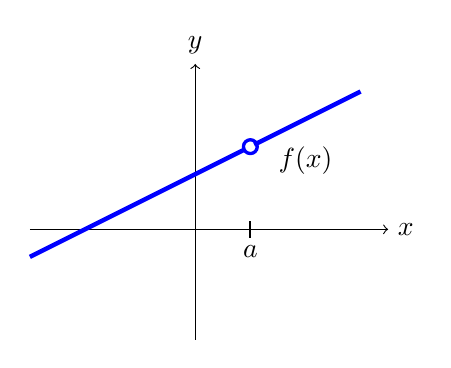
\begin{tikzpicture}[scale =0.7]
\draw[->] (-3,0) -- (3.5,0) node[right,scale=1]{$x$};
\draw[->] (0,-2) -- (0,3) node[above,scale=1]{$y$};
\draw[blue, very thick]  (1,1.5) circle[radius=.125];
\node at (2,1.25) {$f(x)$};

\draw[domain=-3:0.9, smooth, variable=\x, blue, ultra thick] plot ({\x}, {0.5*(\x) +1});
\draw[domain=1.07:3, smooth, variable=\x, blue, ultra thick] plot ({\x}, {0.5*(\x) +1});

\draw[-,thick] (1,0.15) -- (1,-0.15) ;
\node[scale=1] at(1,-0.4) {$a$};
\end{tikzpicture}
}
\end{center}
\end{minipage}
\hspace{0.1cm}
\begin{minipage}{0.3\textwidth}
\begin{center}
\subcaptionbox{}{
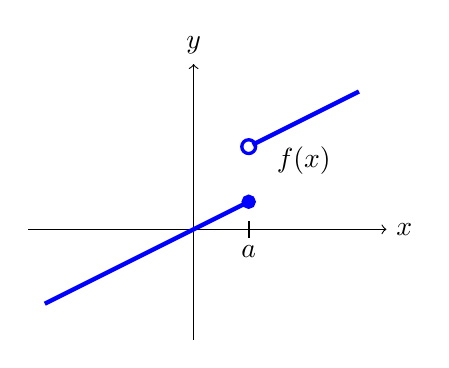
\begin{tikzpicture}[scale =0.7]
\draw[->] (-3,0) -- (3.5,0) node[right,scale=1]{$x$};
\draw[->] (0,-2) -- (0,3) node[above,scale=1]{$y$};

\draw[domain=-2.7:0.9, smooth, variable=\x, blue, ultra thick] plot ({\x}, {0.5*(\x)});
\draw[blue, very thick,fill]  (1,0.5) circle[radius=.1];

\draw[domain=1.07:3, smooth, variable=\x, blue, ultra thick] plot ({\x}, {0.5*(\x)+1});
\draw[blue, very thick]  (1,1.5) circle[radius=.125];
\node at (2,1.25) {$f(x)$};

\draw[-,thick] (1,0.15) -- (1,-0.15) ;
\node[scale=1] at(1,-0.4) {$a$};
\end{tikzpicture}
}
\end{center}
\end{minipage}
\hspace{0.1cm}
\begin{minipage}{0.3\textwidth}

\begin{center}
\subcaptionbox{}{
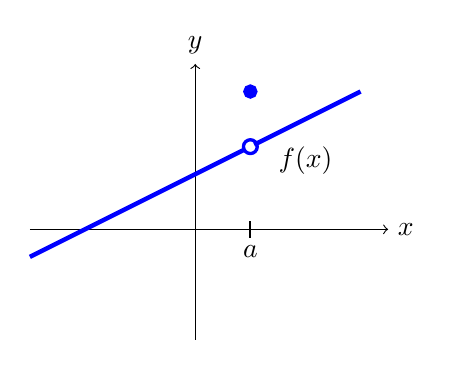
\begin{tikzpicture}[scale =0.7]
\draw[->] (-3,0) -- (3.5,0) node[right,scale=1]{$x$};
\draw[->] (0,-2) -- (0,3) node[above,scale=1]{$y$};
\draw[blue, very thick]  (1,1.5) circle[radius=.125];
\node at (2,1.25) {$f(x)$};
\draw[blue, very thick,fill]  (1,2.5) circle[radius=.1];
\draw[domain=-3:0.9, smooth, variable=\x, blue, ultra thick] plot ({\x}, {0.5*(\x) +1});
\draw[domain=1.07:3, smooth, variable=\x, blue, ultra thick] plot ({\x}, {0.5*(\x) +1});

\draw[-,thick] (1,0.15) -- (1,-0.15) ;
\node[scale=1] at(1,-0.4) {$a$};
\end{tikzpicture}
}
\end{center}
\end{minipage}


\caption{} 
\label{fig:continuity}

\end{figure}
\newpage
%%%Examples%%%
%Example 2.27 from OpenStax; page 182
\begin{example}
Given the the function $f(x)$ below, answer the following questions:
%\vspace{-1cm}
\begin{align*}
f(x) = \left\{ \begin{array}{cc} 
                -x^2+4 & \hspace{2mm} \textrm{if} \quad x\le 3 \\
                4x-8 & \hspace{2mm} \textrm{if} \quad x > 3 \\
                \end{array} \right.
\end{align*}

\begin{enumerate}[leftmargin=*]
    \item Find $f(3)$.
    \vspace{0.5cm}
    \item Find $\lim\limits_{x \to 3^-} f(x)$.
    \vspace{0.5cm}
    \item Find $\lim\limits_{x \to 3^+} f(x)$.
    \vspace{0.5cm}
    \item Checking all \textbf{three conditions} in the definition of \emph{Continuity at a Point}, determine whether the function $f(x)$ is continuous at $x=3$. Justify your answer.
    \vspace{2.5cm}
\end{enumerate}
    %%short answer
    \begin{sol}
    -5;-5;4;discont.
    \end{sol}
    %%solution
    \begin{solL}
    see example 2.27; OpenStax ; page 182.
    
    \end{solL}
\end{example}

%Dave's group exercise 1.5
\begin{example}
Given the the function $f(x)$ below, answer the following questions:
%\vspace{-1cm}
\begin{align*}
f(x) = \left\{ 
                \begin{array}{cc}
                     x+2 &           \hspace{2mm}     \textrm{if}      \quad x < 2 \\
                    x^2 &            \hspace{2mm}     \textrm{if}      \quad x \ge 2 \\
                \end{array}
            \right.
\end{align*}
Using the three conditions, determine if $f(x)$ is continuous at $x=2$. Justify your answer by \textbf{three conditions} for continuity.
\vspace*{\stretch{1.5}}
    %%short answer
    \begin{sol}
    yes.
    \end{sol}
    %%solution
    \begin{solL}
    See solutions to Dave's group exercise 1.5.
    
    \end{solL}
\end{example}


%Dave's 'Differentiability and Continuity' handout 
\begin{example}
Is the function $f(x)=\dfrac{1}{x^2}$ continuous at $x=2$? Justify your answer by checking all \textbf{three conditions} for continuity.
    %%short answer
    \begin{sol}
    yes
    \end{sol}
    %%solution
    \begin{solL}
    Complete solution here.....
    
    \end{solL}
    
\end{example}
\vspace*{\stretch{1.5}}

\begin{example}
Is the function $f(x)=\dfrac{1}{x^2}$ continuous at $x=0$? Justify your answer by checking all \textbf{three conditions} for continuity.
    %%short answer
    \begin{sol}
    no
    \end{sol}
    %%solution
    \begin{solL}
    Complete solution here.....
    
    \end{solL}
    
\end{example}
\vspace*{\stretch{0.5}}


%%%%%%%%%%%%End Examples%%%%%%%%%%%%%%%%%%
%%%%%%%%%%%%%%%End Topic%%%%%%%%%%%%%%%%%%
%%%%%%%%%%%%%%%%Begin Next Topic%%%%%%%%%%%%%%%%%%%%%%%%%%%%%%%


%%%%%%%%%%%%%Begin Next Topic%%%%%%%%%%%%%%%%%%%%%%%%%%%%%%%
\subsection*{Differentiability}%Hoffman (2.2 PROPERTIES AND FORMULAS; Which functions have derivatives?; pg.150)  and Calaway (2.5 Chain Rule ; What if the Derivative Doesn’t Exist?;pg.120)
A function is called \textbf{differentiable} at a point if its derivative exists at that point.\\
\noindent Recall the limit definition of the derivative of the function $f(x)$ at $x=a$:  $f'(x)=\lim\limits_{h \to 0} \displaystyle\frac{f(x+h)-f(x)}{h}$. As we have seen in \emph{Lesson} \ref{limits}, there are certainly some case where a limit does not exist. If this is true for the limit described here, we say that $f(x)$ is nondifferentiable at $x=a$.\\
\vspace{-0.4cm}
\begin{tcolorbox}[title = {Theorem:}]
\begin{center}
IF a function is \textbf{differentiable} at a point, THEN it is \textbf{continuous} at that point.
\end{center}
\end{tcolorbox}


\noindent \textbf{**IMPORTANT**}It is important to clearly understand what is meant by this theorem and what is not meant: 
\begin{itemize}[leftmargin=*]
    \item If the function is \textbf{differentiable} at a point, then the function is automatically \textbf{continuous} at that point.
    \item If the function is \textbf{continuous} at a point, then the function \textbf{may or may not} have a \textbf{derivative} at that point.
    \item If the function is \textbf{not continuous} at a point, then the function is \textbf{not differentiable} at that point.
\end{itemize}

\noindent \textbf{Where can a slope not exist?}
\begin{itemize}
    \item \emph{If there is a sharp corner (cusp) in the graph, the derivative will not exist at that point}. From the graph of the function $f(x)=\abs{x}$ (see Figure \ref{fig:absANDcuberoot}), there are many “tangent lines” that could be drawn at x=a, so there is no “slope” of a unique tangent line at these points. On the left side of the graph, the slope of the line is $=1$. On the right side of the graph, the slope is $+1$. There is no well-defined tangent line at the sharp corner at $x=0$. So the function is \textbf{not differentiable} at that point.
    \item \emph{If the tangent line is vertical, the derivative will not exist}. From the graph of the function $f(x)=x^{1/3}$ (see Figure  \ref{fig:absANDcuberoot}), we can see that the tangent line to this curve at $x=0$ is vertical with undefined slope, which is why the derivative does not exist at $x=0$. 
\end{itemize}
\vspace{-1cm}
\begin{figure}[H]
    \centering
    \begin{minipage}{0.45\textwidth}
        \begin{center}
        \subcaptionbox{}{
            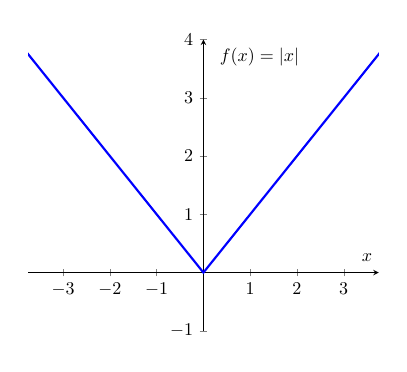
\begin{tikzpicture}[scale=0.65]
                \begin{axis}[
                    axis lines = middle,
                    ymin=-1,ymax=4,
                ]
                    \addplot[color=blue, very thick]{abs(x)};
                    \node at (axis cs:1.2,3.7) {$f(x)=|x|$};
                    \node at (axis cs:3.5,0.25) {$x$};
                \end{axis}
            \end{tikzpicture}
        }
         \end{center}
    \end{minipage}
    \hspace{0.02cm}
    \begin{minipage}{0.45\textwidth}
        \begin{center}
        \subcaptionbox{}{
            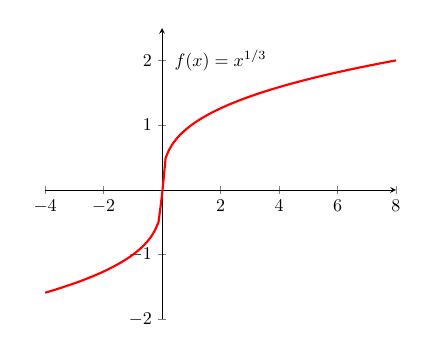
\begin{tikzpicture}[scale=0.65]
                \begin{axis}[
                    axis lines = middle,
                    ymin=-2,ymax=2.5,
                ]
                    \node at (axis cs:2,2) {$f(x)=x^{1/3}$}; \addplot[domain=-4:8,color=red, very thick,samples=100]{x/abs(x)*abs(x)^(1/3)};
                    
                \end{axis}
            \end{tikzpicture}
        }
         \end{center}
    \end{minipage}
    
    \caption{}
    \label{fig:absANDcuberoot}
\end{figure}
\vspace{-0.6cm}
%%%Examples%%%
\begin{example}
Is the function $f(x)=x^2$ differentiable at $x=2$?  Is the function continuous at $x=2$? Justify your answers.
    %%short answer
    \begin{sol}
    yes;yes
    \end{sol}
    %%solution
    \begin{solL}
    Complete solution here.....
    
    \end{solL}
    
\end{example}
\vspace{0.5in}
%%%%%%%%%%%%%%%%%%%%%%%%
\begin{example}
Is the function $f(x)=|x|+1$ differentiable at $x=0$?  Is the function continuous at $x=0$? Justify your answers.
    %%short answer
    \begin{sol}
    no;yes
    \end{sol}
    %%solution
    \begin{solL}
    Complete solution here.....
    
    \end{solL}
    
\end{example}
\vspace{0.5in}
\newpage
\begin{example}
TRUE or False: If $f(x)$ is a continuous function at $x=a$ where $a$ is a constant, then $f(x)$ is a differentiable function at $x=a$.
    %%short answer
    \begin{sol}
    False
    \end{sol}
    %%solution
    \begin{solL}
    Complete solution here.....
    
    \end{solL}
    
\end{example}
\vspace*{\stretch{1}}
\begin{example}
TRUE or False: If $f(x)$ is NOT a continuous function at $x=a$ where $a$ is a constant, then $f(x)$ is NOT a differentiable function at $x=a$.
    %%short answer
    \begin{sol}
    True
    \end{sol}
    %%solution
    \begin{solL}
    Complete solution here.....
    
    \end{solL}
    
\end{example}
\vspace*{\stretch{1}}
\begin{example}
TRUE or False: If $f(x)$ is a differentiable function at $x=a$ where $a$ is a constant, then $f(x)$ is continuous at $x=a$.
    %%short answer
    \begin{sol}
    True
    \end{sol}
    %%solution
    \begin{solL}
    Complete solution here.....
    
    \end{solL}
    
\end{example}
\vspace*{\stretch{1}}

\begin{example}
Given the the function $f(x)=\dfrac{x}{x^2-9}$ , answer the following questions:
%\vspace{-1cm}

\begin{enumerate}[leftmargin=*]
    \item Identify ALL values of $x$ for which $f$ is NOT continous.
    \vspace*{\stretch{1}}
    \item Is it possible to find the slope of the graph at the points found in the previous part? If so, find the slope. If not, explain why it is not possible.
    \vspace*{\stretch{1}}
\end{enumerate}
    %%short answer
    \begin{sol}
    (1) $x=-3$; $x=3$ (2) no.
    \end{sol}
    %%solution
    \begin{solL}
    see example 2.27; OpenStax ; page 182.
    
    \end{solL}
\end{example}
%%%%%%%%%%%%End Examples%%%%%%%%%%%%%%%%%%
%%%%%%%%%%%%%%%End Topic%%%%%%%%%%%%%%%%%%
%%%%%%%%%%End Lesson%%%%%%%%%%%%%%%%%%%%%%
\Closesolutionfile{ans}
\Closesolutionfile{ansL}

%%%Short Answers to Examples%%%
\subsection*{Short Answers to Examples}
\vspace*{\fill}
\begin{multicols}{3}
\input{ans3}
\end{multicols}


